\documentclass{standalone}
\usepackage{tikz}
\usetikzlibrary{positioning}

\begin{document}

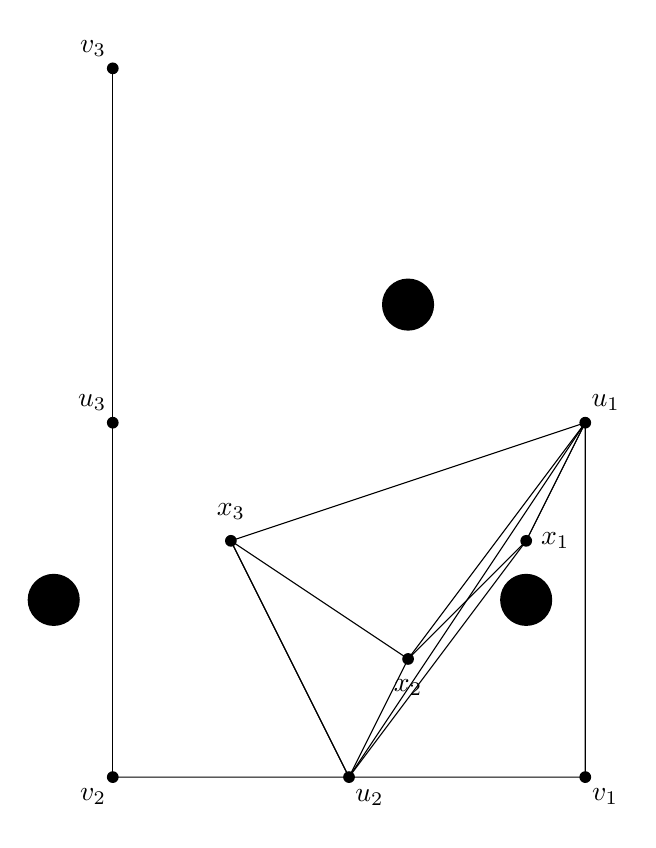
\begin{tikzpicture}[scale=1.5, every node/.style={circle, fill, inner sep=1.5pt}]

% Define coordinates for the main vertices
\coordinate (u1) at (3,0);
\coordinate (u2) at (1,-3);
\coordinate (u3) at (-1,0);
\coordinate (v1) at (3,-3);
\coordinate (v2) at (-1,-3);
\coordinate (v3) at (-1,3);

% Define coordinates for the internal vertices
\coordinate (x1) at (2.5, -1);
\coordinate (x2) at (1.5, -2);
\coordinate (x3) at (0, -1);

% Draw the outer rectangle
\draw (u1) -- (v1) -- (v2) -- (u2) -- cycle;
\draw (u3) -- (v3) -- (v2) -- cycle;

% Draw the internal paths and edges
\draw (u1) -- (x1) -- (x2) -- (x3) -- (u2);
\draw (u1) -- (x3);
\draw (u1) -- (x2);
\draw (u1) -- (x1);
\draw (x3) -- (u2);
\draw (x2) -- (u2);
\draw (x1) -- (u2);

% Place labels for the vertices
\node[label=above right:$u_1$] at (u1) {};
\node[label=below right:$u_2$] at (u2) {};
\node[label=above left:$u_3$] at (u3) {};
\node[label=below right:$v_1$] at (v1) {};
\node[label=below left:$v_2$] at (v2) {};
\node[label=above left:$v_3$] at (v3) {};

\node[label=right:$x_1$] at (x1) {};
\node[label=below:$x_2$] at (x2) {};
\node[label=above:$x_3$] at (x3) {};

% Place labels for the regions
\node at (1.5, 1) {$R_3$};
\node at (-1.5, -1.5) {$R_2$};
\node at (2.5, -1.5) {$R_1$};

\end{tikzpicture}

\end{document}